\section{A sequence of kernel machines with diverging $\mathcal{R}\mathrm{TV}^2$}\label{sec: diverge}
% \begin{tikzpicture}[scale=1.2,every node/.style={font=\small}]
%     % Draw the horizontal rho-axis
%     \draw[->,thick] (0,0) -- (5.3,0) node[right]{$\rho$};
    
%     % Fill the cone region
%     \fill[green!30,opacity=0.5]
%       (0,0) -- (4,1.5)
%       arc[start angle=21.8,end angle=-21.8,radius=4.3] 
%       -- cycle;
    
%     % Dashed lines defining the cone boundary
%     \draw[dashed] (0,0) -- (4,1.5);
%     \draw[dashed] (0,0) -- (4,-1.5);
%     \draw[dashed] (4,1.5) arc[start angle=21.8,end angle=-21.8,radius=4.3];
    
%     % Central blue ray labeled \beta'
%     \draw[->,blue,thick] (0,0) -- (4.2,0.6) node[above]{$\beta'$};
    
%     % Red rays x1 and x2
%     \draw[->,red,thick] (0,0) -- (1.5,0.6) node[left]{$x_1$};
%     \draw[->,red,thick] (0,0) -- (2.5,1.0) node[above]{$x_2$};
    
%     % Purple points x3 and x4 outside the cone
%     \fill[purple] (3.5,2.4) circle (1.6pt) node[right]{$x_3$};
%     \fill[purple] (4.5,3.1) circle (1.6pt) node[right]{$x_4$};
    
%     % Small arc for the angle s at the origin
%     \draw (0.8,0) arc[start angle=0, end angle=22, radius=0.8];
%     \node at (0.9,0.3) {$\mathsf{s}$};
% \end{tikzpicture}
\begin{figure}
    \centering
    %\includegraphics[width=0.5\linewidth]{}
    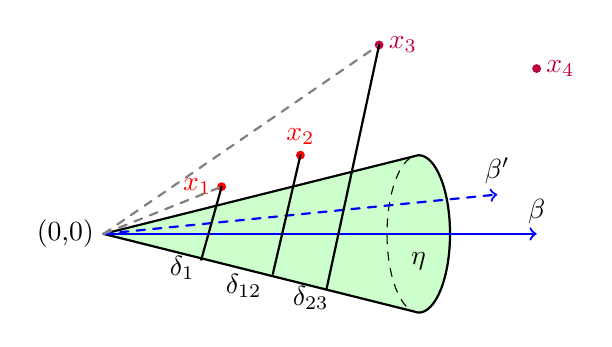
\begin{tikzpicture}[line cap=round,line join=round]

  % Funnel cone
  \path[fill=green!20,draw=black,thick]
    (0,0)                % apex
    -- (4,-1)            % bottom of ellipse
    arc [ start angle=-90, end angle=90,
           x radius=0.4, y radius=1, 
           xshift=4cm, yshift=0cm ]
    -- cycle;            % close back at apex
  
  % (Optional) show the full ellipse in dashed lines for reference
  \draw[dashed] (4,0) ellipse [x radius=0.4, y radius=1];
  
  % Label for the apex
  \node[left] at (0,0) {(0,0)};

  % Small arc for the angle s at the origin
    %\draw (0.5,0) arc[start angle=0, end angle=42, radius=0.6];
    \node at (4.,-0.35) {$\eta$};
  % Blue arrow labeled \beta
  \draw[->,blue,thick]
    (0,0)
    -- (5.5,0) 
    node[above,black] {$\bm{\beta}$};

    \draw[->,blue,dashed,thick]
    (0,0)
    -- (5,0.5) 
    node[above,black] {$\bm{\beta}'$};

    % Red rays x1 and x2
    \fill[red,thick] (1.5,0.6) circle (1.6pt) node[left]{$\bm{x}_1$};
    \fill[red,thick] (2.5,1.0) circle (1.6pt) node[above]{$\bm{x}_2$};
    
    % Purple points \bm{x}3 and x4 outside the cone
    \fill[purple] (3.5,2.4) circle (1.6pt) node[right]{$\bm{x}_3$};
    \fill[purple] (5.5,2.1) circle (1.6pt) node[right]{$\bm{x}_4$};

    \draw[dashed,gray,thick] (0,0) -- (1.5,0.6) node[left]{};
     \draw[dashed,gray,thick] (0,0) -- (3.5,2.4) node[left]{};

    \node at (1.0,-0.43) {$\delta_1$};
    \node at (1.78,-0.658) {$\delta_{12}$};
    \node at (2.63,-0.808) {$\delta_{23}$};
    %\node at (1.24,-0.33) node[left]{$\delta_{}$};
    \draw[thick,black,thick] (1.5,0.6) -- (1.24,-0.33) node[left]{};
    \draw[thick,black,thick] (2.5,1.0) -- (2.15,-0.508) node[left]{};
    \draw[thick,black,thick] (3.5,2.4) -- (2.83,-0.708) node[left]{};

\end{tikzpicture}

    \caption{Illustration of an $(\bm{\beta}, \delta,\eta)$-separated set and a sequence $(\bm{x}_1,\bm{x}_2,\bm{x}_3,\bm{x}_4)$ that satisfy the requirements of the definition. The distances $\delta_1, \delta_{12}, \delta_{23}$ are at least $\delta$ apart.\vspace{-3mm}}
    \label{fig: separated}
\end{figure}

In this section, we show a construction of a family of kernel machines $\curlybracket{f_n \in \cH(\reals^d)}$ such that the corresponding $\cR$-norm, i.e. $\curlybracket{\rtv{f_n}}$, diverges. 

%Assume that $\cX = \reals^d$. Let $\cN(\textbf{0}, 1)$ be a Gaussian distribution over $\cX$. 
% Define the Gaussian RKHS corresponding to a sequence of Mahalanbis matrices $\curlybracket{M_i \succ 0 : M_i \in \sf{Sym}_{+}(\reals^{d \times d})}$ as follows:
% \begin{align*}
%     \cH_n := \curlybracket{f: \cX \to \reals\,\bigg\lvert\, f(\cdot) = \sum_{i = i}^m \alpha_i \cdot K_{M_n}(x_i,\cdot),\, x_i \in \cX_n}
% \end{align*}
First, we state some useful assumptions on probabilist's Hermite polynomial which are easy to verify to hold in general (but surely in odd dimension $d$).

First assumption asserts that Gaussian weighted Hermite polynomial $H_{d+1}(y)e^{-\frac{y^2}{2}}$ has a peak within a finite interval around the origin.
% \begin{assumption}[$\delta$-peak]\label{ass: peak} Fix a dimension $d$. For a given Hermite polynomial $H_{d+1}$ we define an interval $\bracket{-\delta,\delta}$ as a region of $\delta$-peak if the following properties hold:
% \begin{enumerate}
%     \item for every $y > \delta$, $\frac{\partial H_{d+1}(y)e^{-\frac{y^2}{2}}}{\partial y} < 0$,
%     \item for every $y < \delta$, $\frac{\partial H_{d+1}(y)e^{-\frac{y^2}{2}}}{\partial y} > 0$.
% \end{enumerate}
% %a region of $\delta$-peak if     
% \end{assumption}
\begin{assumption}[$\delta$-peak]\label{ass: peak}
Fix a dimension $d$. For a given Hermite polynomial $H_{d+1}$, we call an interval $[-\delta,\delta]$ a region of $\delta$-peak if:
\begin{enumerate}
    \item $\frac{\partial H_{d+1}(y)e^{-\frac{y^2}{2}}}{\partial y} < 0$ for all $y > \delta$
    \item $\frac{\partial H_{d+1}(y)e^{-\frac{y^2}{2}}}{\partial y} > 0$ for all $y < -\delta$
\end{enumerate}
\end{assumption}
Due to exponential decay of the product $H_{d+1}(y)e^{-\frac{y^2}{2}}$, for any odd dimension $d$ note that 
$$\frac{\partial H_{d+1}(y)e^{-\frac{y^2}{2}}}{\partial y} = (H'_{d+1}(y) - yH_{d+1}(y))e^{-y^2/2}$$
where $-yH_{d+1}(y)$ is a polynomial with odd dimension with negative highest term and this implies there exists a $\delta$-peak.

Now, we state a trivial observation on the absolute integral of $H_{d+1}\left( y \right) \, e^{ -\frac{y^2}{2} }$. 
\begin{assumption}[$\epsilon$-safe]\label{ass: safe}
    We say a constant $\epsilon > 0$ is $\epsilon$-safe if $$\int_{[-\epsilon,\epsilon]} \left| H_{d+1}\left( y \right) \, e^{ -\frac{y^2}{2} }\right| \, dy > 0.$$
\end{assumption}
Since $H_{d+1}$ is non-zero polynomial this holds trivially for any $\epsilon > 0$. Furthermore, the integral is increasing with the size of an $\epsilon$-interval. 

With this, we state a useful result on the convergence of a series of evaluations of $H_{d+1}\left( y \right) \, e^{ -\frac{y^2}{2}}$ on distinct points $y \in \reals$. The proof is deferred to \iftoggle{longversion}{\appref{app: useful}}{the supplemental materials}.
% \begin{lemma}\label{lem: safeshift} result that states that for a sufficiently shifted centers/centers there is neighhood using Planchearel-Rotach theorem to show values for each Hermite polynomial is bounded
% \end{lemma}

% \begin{proof}
%     $$H_{d+1}(x) = (d+1)! \sum_{i=0}^{\lfloor (d+1)/2 \rfloor} \frac{(-1)^i x^{d+1-2i}}{(d+1-2i)!i! 2^i}$$
%     Now, we want an interval $[-\epsilon,\epsilon]$ such that
%     \begin{align*}
%         \int_{[-\epsilon,\epsilon]} \left| H_{d+1}\left( y \right) \, e^{ -\frac{y^2}{2} }\right| \, dy > 1
%     \end{align*}
%     Note that,
%     \begin{align*}
%         \int_{[-\epsilon,\epsilon]} \left| H_{d+1}\left( y \right) \, e^{ -\frac{y^2}{2} }\right| \, dy \ge 2\epsilon \cdot (d+1)! \sum_{i=0}^{\lfloor (d+1)/2 \rfloor} \frac{(-1)^i x^{d+1-2i}}{(d+1-2i)!i! 2^i} e^{-\frac{\epsilon^2}{2}}
%     \end{align*}

%     $$H_{d+1}(0) = (-1)^k(2k-1)!!$$
% \end{proof}

\begin{lemma}\label{lem: inter}
Let \( d\ge 0 \) be fixed and let \( H_{d+1}(y) \) denote the Hermite polynomial of degree \( d+1 \). Then for any constant $\rho > 0$, there exists a constant \( \delta_0 > 0 \) (depending only on \( d \)) such that for every \(\delta \ge \delta_0\) we have
\[
\sum_{j=2}^\infty \Bigl| H_{d+1}\bigl(j\delta\bigr) \Bigr|\, e^{-\frac{(j\delta)^2}{2}} < \frac{\rho}{4}.
\]
\end{lemma}


\subsection{Construction of a diverging sequence}

In \secref{sec: setup}, we defined the notions of $(\bm{\beta}, \delta, \eta)$-separated sets of size $n \in \mathbb{N}$. Let $(\bm{x}_1,\bm{x}_2,\ldots,\bm{x}_n)$ be a sequence in this set. Intuitively, any two centers in the sequence are at least $\delta$ apart when projected onto any direction $\bm{\beta}'$ such that $\bm{\beta}^{\mathsf{T}}\bm{\beta}' \ge \norm{\bm{\beta}}\norm{\bm{\beta}'}\eta$ (see \figref{fig: separated} for an illustration). Now, note that in \lemref{lem: cov}, we provided an alternate representation of the $\rtv{f}$ of a function as shown in \thmref{thm: rtv}, specifically the inner integral for each $\bm{\beta} \in \mathbb{S}^{d-1}$ has the form:
$$I_{\sf{inner}}(\bm{\beta}) := \int_{\mathbb{R}} \left| \sum_{i=1}^k \alpha_i H_{d+1}\left( y + \Delta_i \right) e^{ -\frac{(y + \Delta_i)^2}{2} } \right| dy$$
where each $\Delta_i = \bm{x}_1^\mathsf{T}\bm{\beta} - \bm{x}_i^\mathsf{T}\bm{\beta}$ (ignoring the normalization). If the projections $\bm{x}_i^\mathsf{T}\bm{\beta}$ are far apart on the real line $\reals$, noting the absolute decay in the values of $H_{d+1}\left( y \right) \, e^{ -\frac{y^2}{2} }$ outside the region of $\delta$-peak as asserted by \assref{ass: peak}, we can quantify and control contributions of terms corresponding to $j \neq i$ in the inner integral. 

Now, the property holds over a non-trivial cone $\cK(\bm{\beta}) := \curlybracket{\bm{\beta}' \in \mathbb{S}^{d-1}\,|\, \bm{\beta}^{\mathsf{T}}\bm{\beta}' \ge \eta }$ with non-zero volume. Now, noting the \eqnref{eq:transformed_I} which involves the second integral over the unit sphere $\mathbb{S}^{d-1}$, i.e.
$$\int_{\mathbb{S}^{d-1}} \frac{I_{\sf{inner}}(\bm{\beta})}{\sigma^{d+1}} \, d\bm{\beta}$$
is non-trivially positive. Thus, we crucially show along any direction $\bm{\beta}$ in the cone, $I_{\sf{inner}}$ diverges as $k$ grows if the kernel machine $f$ is defined for a sequence of centers from the $(\bm{\beta}, \delta, \eta)$-separated set.

 Now, we state the main theorem of the work. For ease of analysis we assume that the largest eigenvalue of $\mathbf{L}^{-1}$ is upper bounded by 1 which can be easily replaced with appropriate rescaling and choice of the parameters in the statement. 
% \akash{there should be a statement on why separated sets are convex! \exmref{exam: set} can be easily extended for the entire cone!}
 
\begin{theorem}[Diverging $\mathcal{R}\mathrm{TV}^2$]\label{thm: unbounded}
    Consider the Gaussian RKHS $\cH(\reals^d)$ as defined in \eqnref{eq: infinitegauss}. Assume $\epsilon \in (0,1/2]$ be a safe constant (see \assref{ass: safe}). Define \vspace{-2mm}
    \begin{align*}
        \rho :=  \int_{[-\epsilon,\epsilon]} \left| H_{d+1}\left( y \right) \, e^{ -\frac{y^2}{2} }\right| \, dy.\vspace{-2mm}
    \end{align*}
    Fix a unit vector $\bm{\beta} \in \reals^d$, scalars $\eta \ge \frac{\sqrt{3}}{2}$, and $\delta = 3\max\{\epsilon, \delta_0(\rho), \delta'\}$ where $\delta_0(\rho)$ is chosen as per \lemref{lem: inter}, and $\delta'(d)$ as per \assref{ass: peak}. Let $\cX_\infty = \curlybracket{\bm{x}_1,\bm{x}_2,\ldots} \subset \reals^d$ be an infinite sequence such that any subsequence $\Gamma_n = \curlybracket{\bm{x}_1,\bm{x}_2,\ldots, \bm{x}_n}$ is in the $(\bm{\beta}, \delta, \eta)$-separated set of size $n$. Define a function $f \in \cH$ on $\cX_\infty$ that has a representation with an $f$-unbounded combination $\alpha_f$. Then,% and centers $\{x^{(n)}_1,\ldots,x^{(n)}_n\} \in \Gamma_n$. Then, if $s$
    % Let $f_n \in \cH$ be a classifer with combination $\alpha_n$ and centers $\{x^{(n)}_1,\ldots,x^{(n)}_n\} \in \Gamma_n$. Then, if $$
    %$\Gamma_n \subset \cH$ is a $(\beta, \delta, \eta)$-separated set of size $n$.
    \begin{align}
        \rtv{\{f_n\}} \to \infty
    \end{align}
\end{theorem}

\begin{proof}
    %\akash{you start with fixing some $\epsilon >0$ for which you get some $\rho$, which you use to pick one bound on $\delta$. Either adjust $\eta$ for $\delta$ or vice versa.  I mean if $\eta$ is large then $\delta$ needs to be large as well}
    First, we rewrite \eqnref{eq:transformed_I} for the $\cR$-norm of the function $f_k$ as follows
    \begin{align*}
        \rtv{f_k} &= \frac{1}{|\det \mathbf{L}| \sqrt{2\pi}} \int_{\mathbb{S}^{d-1}} \frac{1}{\sigma^{d+1}} \int_{\mathbb{R}} \left| \sum_{i=1}^k \alpha_i H_{d+1}\left( y + \Delta_i \right) e^{ -\frac{(y + \Delta_i)^2}{2} } \right| dy \, d\bm{\beta} 
    \end{align*}
    with the inner integral \vspace{-2mm}
    \[I_{\sf{inner}}(\bm{\beta}) = \int_{\reals} \left| \sum_{i=1}^k \alpha_i \, H_{d+1}\left( y + \Delta_i \right) \, e^{ -\frac{(y + \Delta_i)^2}{2} } \right| \, dy
\]
where:
\[
\Delta_1 = 0,\,\,\Delta_i = \frac{a_1 - a_i}{\sigma} = \frac{\bm{x}_1^\mathsf{T}\bm{\beta} - \bm{x}_i^\mathsf{T}\bm{\beta}}{\|\mathbf{L}^{-\mathsf{T}}\bm{\beta}\|}
\quad \text{for } i = 2, 3, \ldots, k.
\]
First, define the cone $\cK$ wrt $\bm{\beta}$ and $\eta$ as stated in the theorem statement, i.e.
\begin{align*}
    \cK := \curlybracket{\bm{\beta}' \in \mathbb{S}^{d-1}\,|\, \bm{\beta}'^{\mathsf{T}} \bm{\beta} \ge \eta}
\end{align*}
Note that the volume $\vol{\cK} > 0$ implying that 
\begin{align}
    \int_{\mathbb{S}^{d-1}} \frac{1}{\sigma^{d+1}} \, d\bm{\bm{\beta}} \ge  \int_{\cK} \frac{1}{\sigma^{d+1}} \, d\bm{\beta} = (\star) \label{eq: cone}
\end{align}
    Note that $\mathbf{M} = \mathbf{L}^\mathsf{T}\mathbf{L}$. We assume that the $\mathbf{M}$ is symmetric and PSD, implying that singular values of $\mathbf{L}$ are \tt{exactly} the square root of the eigenvalues of $\mathbf{M}$, i.e
    \[ \sigma_i(\mathbf{L}) = \sqrt{|\lambda_i(\mathbf{M})|}\]
    \looseness-1 But since $\mathbf{L}$ is invertible implying the singular values if $\mathbf{L^{-1}}$ are inverses to singular values of $\mathbf{L}$, i.e. $\sigma_i(\mathbf{L}^{-1}) = \frac{1}{\sigma_i(\mathbf{L})}$.
    Thus, we can rewrite \eqnref{eq: cone} as
    \begin{align}
     (\star) =  \int_{\cK} \frac{1}{\sigma_{\max}(\mathbf{L}^{-1})^{d+1}} \, d\bm{\beta} \ge \int_{\cK} \sigma_{\min}(\mathbf{L})^{d+1} \, d\bm{\beta} = \int_{\cK} \lambda_{\min}(\mathbf{M})^{\frac{(d+1)}{2}} \, d\bm{\beta} =  \lambda_{\min}(\mathbf{M})^{\frac{(d+1)}{2}} \vol{\cK} > 0 \label{eq: vol}
    \end{align}
    Now, we will show for any $\bm{\beta}' \in \cK$, there is a non-trivial lower bound on $I_{\sf{inner}}(\bm{\beta}')$. Note that by definition, $\Gamma_n$ is in the $(\bm{\beta}',\delta)$-separated set. 

    Hence, for all $i,j = 2, 3, \ldots$
    \begin{align*}
        |\Delta_i - \Delta_j| \ge \delta
    \end{align*}
    Define the neighborhoods $\curlybracket{N_i}$ for the safe constant $\epsilon$ as follows
    $$N_i := \bracket{-\Delta_i - \epsilon, -\Delta_i + \epsilon}.$$
    %But using \lemref{lem: safeshift}, we know that there exists $\epsilon > 0$ and 
    Now, consider the integral on the neighborhood $N_i$:
    \begin{align*}
        &\int_{N_i} \left| \sum_{i=1}^k \alpha_i \, H_{d+1}\left( y + \Delta_i \right) \, e^{ -\frac{(y + \Delta_i)^2}{2} } \right| \, dy \\
        &\ge \int_{N_i} \left|\alpha_i \, H_{d+1}\left( y + \Delta_i \right) \, e^{ -\frac{(y + \Delta_i)^2}{2} } \right| \, dy - \underbrace{\int_{N_i} \left| \sum_{j=1, j \neq i}^k \alpha_j \, H_{d+1}\left( y + \Delta_j \right) \, e^{ -\frac{(y + \Delta_j)^2}{2} } \right| \, dy}_{=: \large{\theta_i}}\\ 
        &\hspace{100mm}\text{(triangle inequality)}\\
        &\ge |\alpha_i| \int_{[-\epsilon,\epsilon]} \left|H_{d+1}\left( y \right) \, e^{ -\frac{y^2}{2} } \right| \, dy - \theta_i \hspace{38.5mm}\text{(change of variable)} \\ 
        &\ge |\alpha_i| \rho - \theta_i \hspace{85mm}\text{(definition of $\rho$)}
    \end{align*}

    Summing over each $i = 1, 2, \ldots k$, we get
    \begin{align}
        I_{\sf{inner}} &\ge \sum_{i = 1}^k \int_{N_i} \left| \sum_{i=1}^k \alpha_i \, H_{d+1}\left( y + \Delta_i \right) \, e^{ -\frac{(y + \Delta_i)^2}{2} } \right| \, dy \nonumber\\
        & \ge \rho \sum_{i=1}^k |\alpha_i| - \sum_{i=1}^k \theta_i \label{eq: diff}
    \end{align}
     %\akash{show why the negative term is bounded}
    Now, we will show how to bound the sum $\sum_{i=1}^k \theta_i$.%\akash{show why $|i-j|\delta$ diff work below}
    \paragraph{Bounding $\theta_k$:} First note that, we can bound each $\theta_i$ as follows\vspace{-5mm}
    \allowdisplaybreaks
    \begin{center}
    \begin{align*}
        \theta_i &= \int_{N_i} \left| \sum_{j=1, j \neq i}^k \alpha_j \, H_{d+1}\left( y + \Delta_j \right) \, e^{ -\frac{(y + \Delta_j)^2}{2} } \right| \, dy \\ &\le  \sum_{j=1, j \neq i}^k \int_{N_i} \left|  \alpha_j \, H_{d+1}\left( y + \Delta_j \right) \, e^{ -\frac{(y + \Delta_j)^2}{2} } \right| \, dy \quad &\text{(triangle inequality)}\\
        &\le  \sum_{j=1, j \neq i}^k \int_{\bracket{-\epsilon,\epsilon}} \left|  \alpha_j \, H_{d+1}\left(-\Delta_i + y + \Delta_j \right) \, e^{ -\frac{(-\Delta_i + y + \Delta_j)^2}{2} } \right| \, dy &\text{(change of variable)}\\
        & \le \sum_{j=1, j \neq i}^k |\alpha_j| \int_{\bracket{-\epsilon,\epsilon}}  \left| H_{d+1}\left( |i-j|\delta \right) \, e^{ -\frac{(|i-j| \delta)^2}{2} } \right| \, dy \quad &\text{($\delta$-peak)} \\
        %& \le \sum_{j=1, j \neq i}^k |\alpha_j| \int_{N_i}  \left| H_{d+1}\left( j\delta \right) \, e^{ -\frac{(j \delta)^2}{2} } \right| \, dy \\
        & \le 2 \epsilon \sum_{j=1, j \neq i}^k |\alpha_j| \left|H_{d+1}\left( |i-j|\delta \right)\right| \, e^{ -\frac{(|i-j| \delta)^2}{2} } \\
        & \le \sum_{j=1, j \neq i}^k |\alpha_j| \left|H_{d+1}\left( |i-j|\delta \right)\right| \, e^{ -\frac{(|i-j| \delta)^2}{2} } \quad &\text{($\epsilon \le 1/2$)}
        %&\le (k-1) H_{d+1}\left( 2\delta \right) \, e^{ -\frac{(2 \delta)^2}{2} } \sum_{j=1}^k |\alpha_j| \\
        %& \le C_{2\delta} (k-1) \sum_{i=1}^k |\alpha_i|
    \end{align*}
    \end{center}
    To simplify $-\Delta_i + y + \Delta_j$ for a choice of $y \in \bracket{-\epsilon,\epsilon}$, we assume that indices of the projections $\Delta_i$ for $i = 1,2, \ldots$ are arranged in ascending order in their values on the real line. Since each consecutive projections are at least $\delta$ apart, we can bound $|-\Delta_i + y + \Delta_j| > (|i-j| - 1/3)\delta$. Since Hermite polynomials in even dimension, i.e. $d+1$, are even 
    \begin{align*}
      \left|H_{d+1}\left(-\Delta_i + y + \Delta_j \right) \, e^{ -\frac{(-\Delta_i + y + \Delta_j)^2}{2}}\right| \le \left| H_{d+1}\left((|i - j| - 2/3)\delta\right) e^{ -\frac{((|i - j| - 2/3)\delta)^2}{2}} \right|  
    \end{align*}
    For simplification, we have omitted the $-(2/3)\delta$ additive term in the equation above.

    Summing over each $i = 1,\ldots,k$
    \begin{align*}
        \sum_{i=1}^k \theta_k &= \sum_{i=1}^k \int_{N_i} \left| \sum_{j=1, j \neq i}^k \alpha_j \, H_{d+1}\left( y + \Delta_j \right) \, e^{ -\frac{(y + \Delta_j)^2}{2} } \right| \, dy \\
        &\le \sum_{i=1}^k \sum_{j=1, j \neq i}^k |\alpha_j| \left|H_{d+1}\left( |i-j|\delta \right)\right| \, e^{ -\frac{(|i-j| \delta)^2}{2} }\\
        &\le 2\paren{\sum_{j=1}^{k}  \left|H_{d+1}\left( j\delta \right) \right|\, e^{ -\frac{(j \delta)^2}{2} }} \sum_{i=1}^k |\alpha_i|
    \end{align*}
    Using \lemref{lem: inter}, we can rewrite \eqnref{eq: diff}
    \begin{align}
        I_{\sf{inner}} \ge \rho \sum_{i=1}^k |\alpha_i| - 2\paren{\sum_{j=2}^k  \left|H_{d+1}\left( j\delta \right)\right| \, e^{ -\frac{(j \delta)^2}{2} }} \sum_{i=1}^k |\alpha_i| \ge \frac{\rho}{2}\sum_{i=1}^k |\alpha_i| 
    \end{align}
    % Now, in the limiting case
    % \begin{align*}
    %     \lim_{k \to \infty}  I_{\sf{inner}}(\bm{\beta}') \ge \lim_{k \to \infty} \rho \sum_{i=1}^k |\alpha_i| - \lim_{k \to \infty} \sum_{i=1}^k \theta_k \ge \frac{\rho}{2} \norm{\alpha_f}_{\ell_1}
    % \end{align*}
    % Since $\rho > 0$, we have $\frac{\rho}{2} \norm{\alpha_f}_{\ell_1} \to \infty$ as $ \norm{\alpha_f}_{\ell_1}$ is unbounded.

    % Since $\bm{\beta}'$ was arbitrarily picked from the cone $\cK$, for all $\bm{\beta}' \in \cK$
    % \begin{align}
    %      \lim_{k \to \infty}  I_{\sf{inner}}(\bm{\beta}') \to \infty \label{eq: limit}
    % \end{align}
    \noindent Now, note that using \eqnref{eq: cone} and \eqnref{eq: vol}
    \begin{align*}
        \rtv{f_k} &\ge \frac{1}{|\det \mathbf{L}| \sqrt{2\pi}} \int_{\cK} \frac{1}{\sigma^{d+1}} \int_{\mathbb{R}} \left| \sum_{i=1}^k \alpha_i H_{d+1}\left( y + \Delta_i \right) e^{ -\frac{(y + \Delta_i)^2}{2} } \right| dy \, d\bm{\beta} \\
        & \ge \frac{1}{|\det \mathbf{L}| \sqrt{2\pi}} \int_{\cK} \frac{1}{\sigma^{d+1}}  \paren{\frac{\rho}{2}\sum_{i=1}^k |\alpha_i| } \, d\bm{\beta}\\
        & \ge \paren{\frac{1}{|\det \mathbf{L}| \sqrt{2\pi}} \lambda_{\min}(\mathbf{M})^{\frac{(d+1)} {2}} \vol{\cK}} \cdot\paren{\frac{\rho}{2}\sum_{i=1}^k |\alpha_i| }
    \end{align*}
    Now, in the limiting case
    \begin{align*}
        \lim_{k \to \infty} \rtv{f_k} &\ge \paren{\frac{1}{|\det \mathbf{L}| \sqrt{2\pi}} \lambda_{\min}(\mathbf{M})^{\frac{(d+1)} {2}} \vol{\cK}} \lim_{k \to \infty} \paren{\frac{\rho}{2}\sum_{i=1}^k |\alpha_i| } \\
        & =  \paren{\frac{1}{|\det \mathbf{L}| \sqrt{2\pi}} \lambda_{\min}(\mathbf{M})^{\frac{(d+1)} {2}} \vol{\cK}} \cdot \frac{\rho}{2} \norm{\alpha_f} \to \infty
    \end{align*}
    Hence the claim of the theorem has been proven.
\end{proof}
%\akash{ should fix $\rho > 1$, it depends on choice of $\epsilon$ which will affect $\delta$ as well}
    
    
    
    
    % Now, consider the following bound
    % \begin{align*}
    %     \frac{1}{\norm{\mathbf{L}^{-\mathsf{T}}\bm{\beta}}} \le \frac{1}{\sigma_{\min}(\mathbf{L}^{-1})} = \sigma_{\max}(\mathbf{L}) = \sqrt{\lambda_{\max}(\mathbf{M})}
    % \end{align*}
    % Thus, we can write 
    % \[
    % \cA \le \lambda_{\max}(\mathbf{M})^{\frac{d+1}{2}} \cdot \int_{\mathbb{S}^{d-1}} \,\mathrm{d}\bm{\beta} = \lambda_{\max}(\mathbf{M})^{\frac{d+1}{2}} \cdot\frac{2\pi^{\frac{d}{2}}}{\Gamma\paren{\frac{d}{2}}}
    % \]
    % where $\Gamma$ is a \textbf{Gamma} function.
    % Since $\lambda_{\max}(\mathbf{M})$ is a bounded value, we note that $\cA$ is bounded above by a constant that depends on the largest eigenvalue of $\mathbf{M}$ and the dimension $d$.
    % \end{proof}
% \end{proof}

